\section{Multi-Rotor Control}\label{sec:controlLaw}

A ferrous particle in the strong static field of an MRI becomes magnetized, and its magnetization magnitude asymptotically approaches the saturation magnetization $\mathbf{M}_s$ per unit volume of the material.  The MRI gradient coils  produce a magnetic field  $\mathbf{B}_g(t)$. This field exerts 
 on the ferrous particle the force 
\begin{equation}
\mathbf{F}(t) = v\left( \mathbf{M}_s
\cdot \nabla \right) \mathbf{B}_g(t). \label{eq:forceOnDipole}
\end{equation}
Here $v$ is the magnetic volume of the material.  The magnetic field $\mathbf{B}_g(t)$ is designed to produce three independent gradients:
\begin{equation}
\left[ F_x,F_y, F_z \right]^\intercal\!\!(t)= v M_{sz}\left[ 
   \frac{ \partial B_{gz}}{\partial x}, 
   \frac{ \partial B_{gz}}{\partial y},
   \frac{ \partial B_{gz}}{\partial z} 
   \right]^\intercal\!\!\!\!(t)
\label{eq:applicableForces}
\end{equation}
Here it has been reasonably assumed that $M_{sz} \gg M_{sx}, M_{sy}$.
These gradients apply three independent forces on any ferromagnetic spheres inside the MRI.  
 \begin{figure}
 \centering
% \vspace{-1em}
\begin{overpic}[width = 0.85\columnwidth]{Schematic2.pdf}\end{overpic}
 \vspace{-1em}
\caption{
\label{fig:Schematic}
MRI-powered, single-DOF rotor with gear for power transmission.
}
\vspace{-1.5em}
\end{figure}
This paper investigates rotors that constrain the $i$th ferromagnetic sphere to rotate about an axis $\mathbf{a}_i$ with a moment arm of length  $r_i$, as shown in Fig.~\ref{fig:Schematic}.  The rotor's configuration is fully described  by its angular position and velocity $[\theta_i, \dot{\theta}_i]^\intercal$. The configuration space of all $n$ rotors is $\R^{2\times n}$,  and the dynamic equations are

\begin{equation}
J_i\ddot{\theta}_i(t) = -b_i\dot{\theta}_i(t) -\tau_{f_i}-\tau_{\ell_i} + r_i \mathbf{F}\cdot \mathbf{p}_i(t)
\label{eq:rotorDynamics}
\end{equation}
Here $J_i$ is the moment of inertia, $b_i$ the coefficient of viscous friction,  $\tau_{f_i}$ the summation of all non-viscous friction terms seen by the input,  and $\tau_{\ell_i}$ the load torque. The rotor torque is the magnetic force projected  to a vector tangent to the ferrous sphere's positive direction of motion, $r_i \mathbf{F}\cdot \mathbf{p}_i(t)$
Actuator torque is maximized when $\mathbf{F}(t) = g_{M}V M_{sz}\sgn(\mathbf{p}_i(t)) $, where  $g_{M}$ is the maximum gradient.

There are two standard actuator control tasks: position and velocity control. 
%Given $q(0)\in \R^{2\times n}$, and $\bm{\theta}_{\textrm{goal}}\in\R^n$ the position control problem is to find inputs $\mathbf{F}(t)$ such that for any $q(0)$ and $q_{\textrm{goal}}$, 
The position control problem is to find inputs $\mathbf{F}(t)$ such that for any $\bm{\theta}(0)$ and $\bm{\theta}_{\textrm{goal}}$, 
\begin{equation}\lim_{t \to \infty}\sum_{i=1}^n \norm{\begin{bmatrix}\theta_i(t)\\ \dot{\theta}_i(t)\end{bmatrix}-\begin{bmatrix}\theta_{\textrm{goal},i}\\ 0 \end{bmatrix} }_2 = 0.
\end{equation}
This section starts with the simpler velocity control problem
\begin{equation}
\lim_{t \to \infty}\sum_{i=1}^n \norm{ \dot{\theta}_i(t)- \omega_i }_2 = 0,
\end{equation}
where $\omega_i \in \R$ is the desired angular velocity of each rotor. After solving the velocity control problem in Sec. \ref{subsec:ControlLyapunov},   Section \ref{subsec:PositionControl} uses an outer control loop to stabilize position.




\subsection{Open-Loop Multi-Actuator Control}
Before considering closed-loop control, it is worthwhile to determine what can be achieved in open-loop and to examine related performance limitations.  In this context, one method to independently control multiple rotors uses the magnetic field gradients to make the rotors revolve around \emph{orthogonal} axes. For notational simplicity, assume the rotors rotate about the world $x,y,z$ axes.
With $n\le3$ orthogonal rotors,  open-loop control signals can rotate some rotors at constant velocities, and move the remaining rotors to steady-state positions.  For instance, the control law
\begin{equation}
\nabla  \mathbf{B}_g(t) = g_{M} \left[  \cos(t), \sin(t), 0  \right]^\intercal
\end{equation}
rotates the $z$-axis rotor in the positive direction at 1 rad/s  and places the $x$ and $y$ rotors in steady-state positions.

To simultaneously rotate up to three orthogonal rotors, the gradient can be rotated at angular frequency $\omega$ around the vector $\bm{\phi} = \dfrac{[\phi_x,\phi_y,\phi_z]^\intercal}{\sqrt{\phi_x^2+\phi_y^2+\phi_z^2}}$, where $\phi_i \in \{-1,0,1\}$ is the desired rotation of the $i$th axis. This gives the control law
\begin{align}
\label{eq:OpenLoopControlRotors3}
\nabla  \mathbf{B}_g(t) &= g_{M} R_{\bm{\phi},\omega t} \cdot \bm{\phi}_{\perp}.
\end{align}
Here $\bm{\phi}_{\perp}$ is a vector perpendicular to $\bm{\phi}$ and $R_{\bm{\phi},\omega t}$ is the rotation matrix that rotates the angle $\omega t$ about the axis $\bm{\phi}$.  Control law  \eqref{eq:OpenLoopControlRotors3} with three orthogonal rotors has 27 possible outputs.  Figure \ref{fig:OpenLoopRotationsArrow} shows three representative control inputs.  The 2D projections show how rotating the magnetic field around different $\bm{\phi}$ vectors rotates one, two, or three rotors simultaneously.

 \begin{figure}
 \centering
 \begin{minipage}{0.4\linewidth}
\begin{overpic}[width = \columnwidth]{OpenLoopRotationsArrow3.pdf}
\put(54,9){$\theta_x$}
\put(67,53){$\theta_y$}
\put(12,85){$\theta_z$}
\end{overpic}
\end{minipage}~~\begin{minipage}{0.58\linewidth}
\begin{overpic}[width=0.3\textwidth]{projForOpenLoopg2}\put(12,85){$\theta_x$}\end{overpic}
\begin{overpic}[width=0.3\textwidth]{projForOpenLoopg1}\put(12,85){$\theta_z$}\end{overpic}
\begin{overpic}[width=0.3\textwidth]{projForOpenLoopg3}\put(12,85){$\theta_y$}\end{overpic}\\
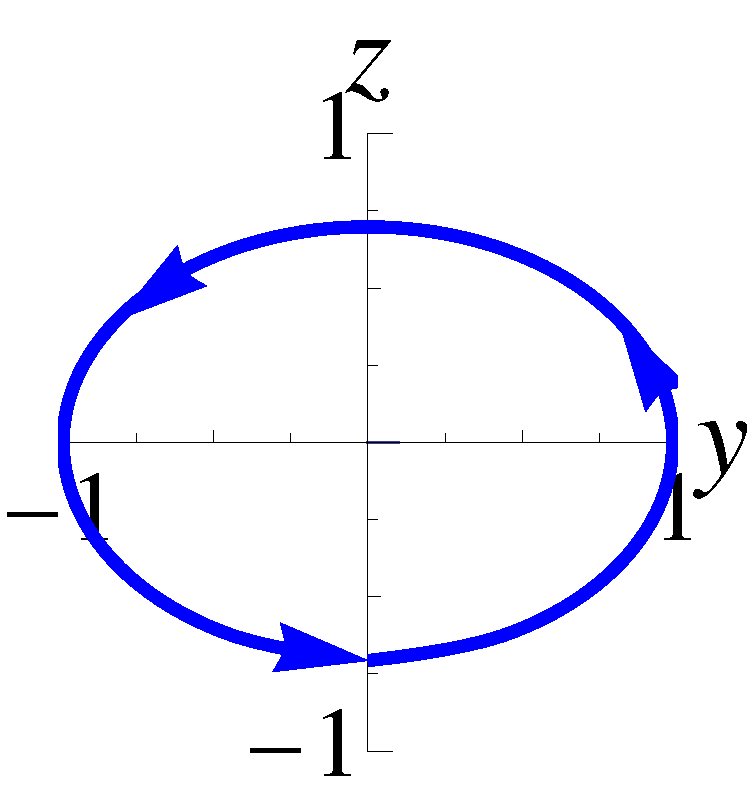
\includegraphics[width=0.3\textwidth]{projForOpenLoopb2}
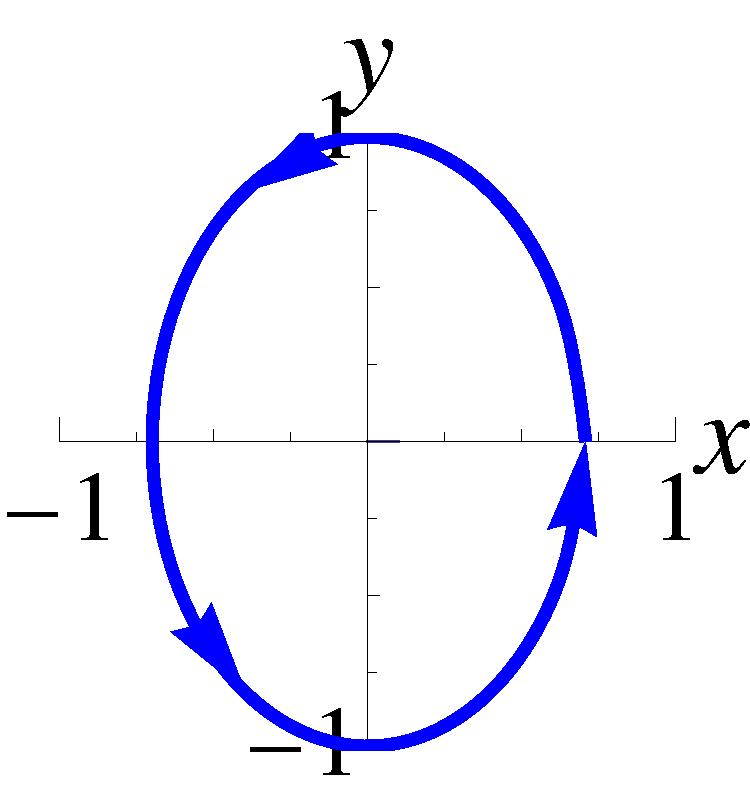
\includegraphics[width=0.3\textwidth]{projForOpenLoopb1}
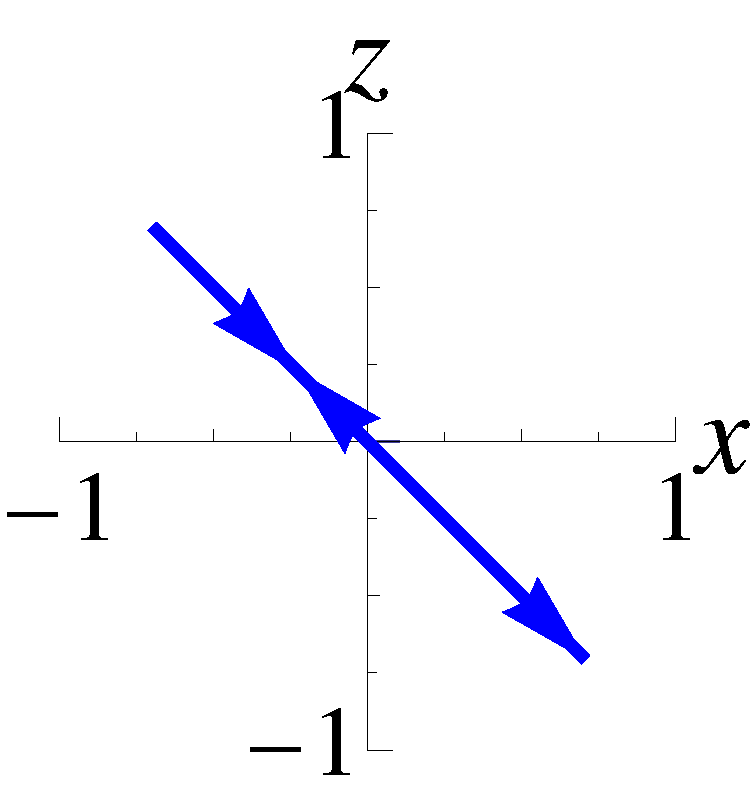
\includegraphics[width=0.3\textwidth]{projForOpenLoopb3}\\
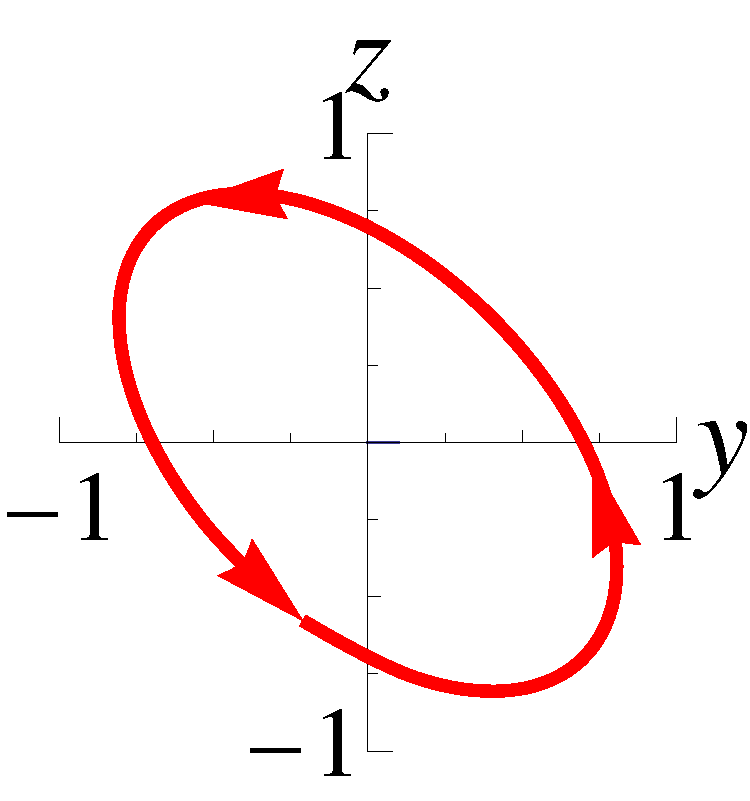
\includegraphics[width=0.3\textwidth]{projForOpenLoopr2}
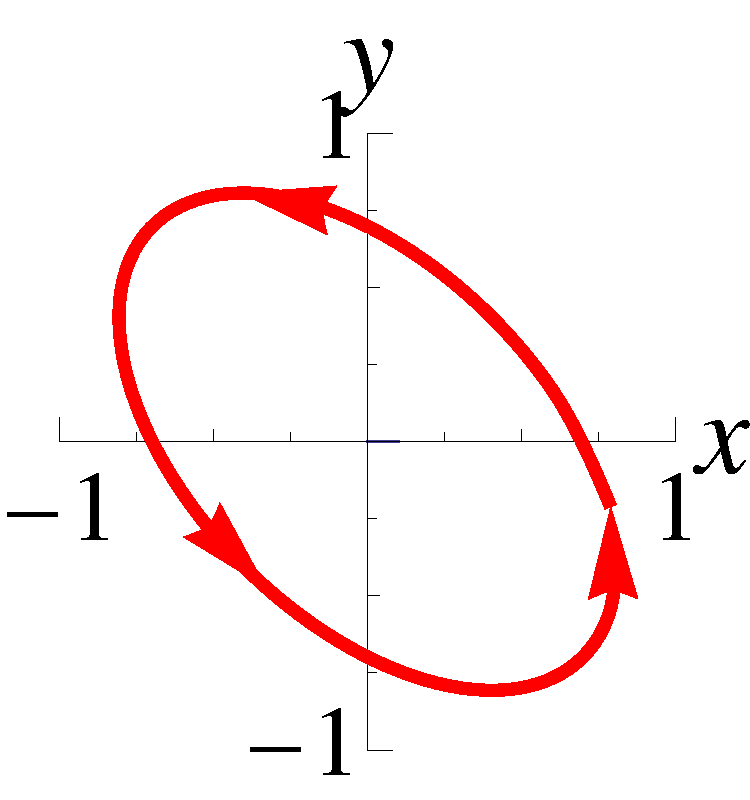
\includegraphics[width=0.3\textwidth]{projForOpenLoopr1}
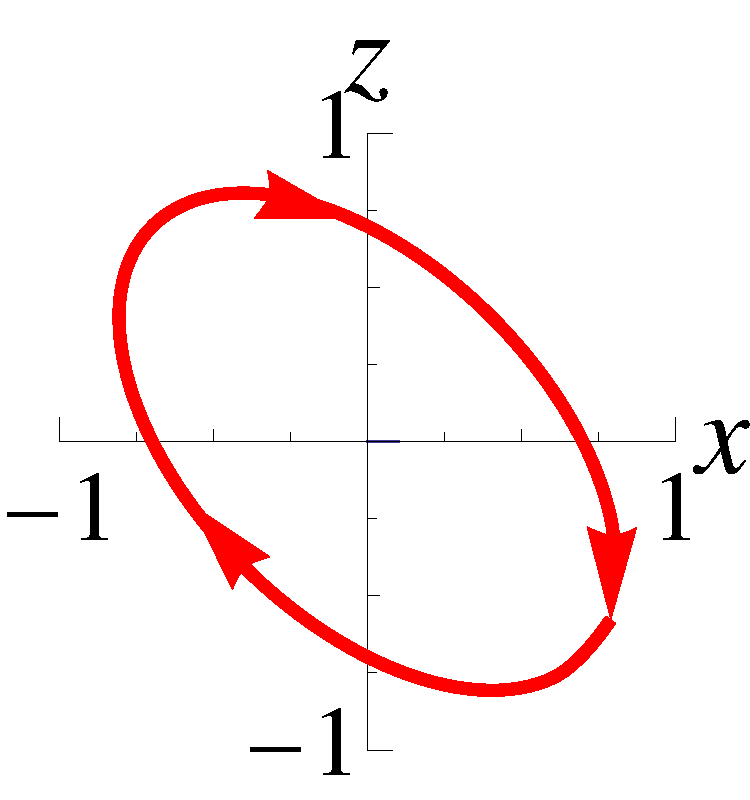
\includegraphics[width=0.3\textwidth]{projForOpenLoopr3}\\
\end{minipage}
\vspace{-1.75em}
\caption{
\label{fig:OpenLoopRotationsArrow}
The open-loop control law  \eqref{eq:OpenLoopControlRotors3} for three orthogonal axes has 27 possible outputs corresponding with: only one rotor spinning (green), two rotors spinning (blue), all three spinning (red), or none spinning. At right are projections onto the three coordinate axes. \href{http://youtu.be/nzym0mABaKY}{See video attachment for experimental verification.}
}\vspace{-2em}
\end{figure}

As demonstrated in these examples, open-loop control has several limitations. For example, rotor velocities are coupled and position control is not possible. In addition, the approach is limited to at most three rotors since their axes must be orthogonal. Furthermore, as shown in the \href{http://youtu.be/nzym0mABaKY}{video attachment}, cyclic slipping of the rotor due to applied load or perturbations is possible. Closed-loop control, described in the following subsection, can eliminate these limitations. 
  \begin{figure*}
\subfloat[positions, 4 rotor  control]{\begin{overpic}[height = 0.206\linewidth]{PositionConverge4state.pdf}\end{overpic}}
\subfloat[control inputs, 4 rotor control]{\begin{overpic}[height = 0.206\linewidth]{PositionConverge4control.pdf}\end{overpic}}
\subfloat[positions, 24 rotor control]{\begin{overpic}[height = 0.206\linewidth]{PositionConverge24state.pdf}\end{overpic}}\vspace{-1.em}\\
\vspace{-1.2em}
\subfloat[positions, 4 rotor  control, no load]{\begin{overpic}[height = 0.206\linewidth]{PositionConverge4stateNoload.pdf}\end{overpic}}
\subfloat[control inputs, 4 rotor control, no load]{\begin{overpic}[height = 0.206\linewidth]{PositionConverge4controlNoload.pdf}\end{overpic}}
\subfloat[positions, 50 rotor control]{\begin{overpic}[height = 0.206\linewidth]{PositionConverge50state.pdf}\end{overpic}}\\
\caption{\label{fig:PositionControlSim}Simulated position control of multiple non-parallel rotors.  }
\vspace{-1.75em}
\end{figure*}
\subsection{Closed-Loop Multi-Actuator Velocity Control }\label{subsec:ControlLyapunov}
   To enable robust, multi-axis control, a closed-loop controller can be designed using a control-Lyapunov function~\cite{Artstein1983}.  The control law selects the three magnetic gradients that decrease the sum of squared velocity error. There are configurations where no combination of velocity gradients will decrease this error, but it is always possible to apply a non-zero gradient without increasing the sum squared error. Any non-zero gradient will move the rotors to a new configuration where the error can be decreased. This technique is inspired by work on controlling many mobile robots with a uniform control signal~\cite{Becker2012k}.
  For ease of analysis, simplified rotor dynamics will be used: 
   \begin{equation}
\ddot{\theta}_i(t) =   \frac{r_i}{J_i} \mathbf{F}(t)\cdot \mathbf{p}_i(t).
\label{eq:rotorDynamicsSimple}
\end{equation}
   In all simulations the full dynamic model \eqref{eq:rotorDynamics} is used.
   
   Given $n$ non-parallel rotors and desired angular velocities $\omega_i$, a suitable Lyapunov function can be defined as the sum squared velocity error:
   \begin{align}
   \label{eq:LyapunovFunction}
   V(\bm{\theta},\dot{\bm{\theta}},t) &= \frac{1}{2} \sum_{i=1}^n \left(  \omega_i - \dot{\theta}_i(t)\right)^2 
      \end{align}
      \begin{align}
   \label{eq:LyapunovFunctionD}
   \dot{V}(\bm{\theta},\dot{\bm{\theta}},t) &=  \sum_{i=1}^n \left( \omega_i - \dot{\theta}_i(t)  \right) \ddot{\theta}_i(t)   \nonumber \\
  &=  \mathbf{F}(t)\cdot \sum_{i=1}^n \left(  \omega_i - \dot{\theta}_i(t) \right) \frac{r_i}{J_i} \mathbf{p}_i(t)
   \end{align}
Note that $V(\bm{\theta},\dot{\bm{\theta}},t)$ is positive definite, zero only at the target velocity, and radially unbounded. The following controller makes $ \dot{V}(\bm{\theta},\dot{\bm{\theta}},t) $ negative semi-definite:
\begin{equation}
\label{eq:velocityControlPolicy}
\mathbf{F}(t) = -g_{M}v_i  M_{sz}\left(  \sum_{i=1}^n \left(  \omega_i - \dot{\theta}_i(t) \right) \frac{r_i}{J_i}  \mathbf{p}_i(t)    \right)
\end{equation}
 For such an $\mathbf{F}(t)$,
   \begin{align*}
  \dot{V}(\bm{\theta},\dot{\bm{\theta}},t) &=  -  g_{M}v_i  M_{sz}\left( \sum_{i=1}^n \left(  \omega_i - \dot{\theta}_i(t) \right) \frac{r_i}{J_i}  \mathbf{p}_i(t) \right)^2.
   \end{align*}
Notice that  $\dot{V}(\bm{\theta},\dot{\bm{\theta}},t)\le0$, but there exists a subspace of $[\bm{\theta}, \dot{\bm{\theta}}]^\intercal$ where $\dot{V}(\bm{\theta},\dot{\bm{\theta}},t)=0$.  Because this derivative is negative semi-definite, the system is stable, but not necessarily asymptotically stable.  To prove asymptotic stability requires proving that the invariant set contains only the rotors moving at the desired angular velocity.  

Control law \eqref{eq:velocityControlPolicy} is modified as follows:
   \begin{align}
\mathbf{f} & = \sgn\!\left(  -\sum_{i=1}^n \left(  \omega_i - \dot{\theta}_i(t) \right) \frac{r_i}{J_i}  \mathbf{p}_i(t)    \right)\nonumber\\
\mathbf{F}(t) &=g_{M}v_i M_{sz}\begin{cases} [1,1,1]^\intercal &\mbox{if } \mathbf{f} = 0 \mbox{ and } \dot{\bm{\theta}} \ne \bm{\omega} \\ 
					       \mathbf{f} & \mbox{else } \end{cases}
					       \label{eq:velocityControlPolicyInv}
   \end{align}
The \emph{signum function} $\sgn(\cdot)$ returns the sign of the argument, or 0 if the argument is zero. 
This ensures that the only invariant state is the target velocity $ \dot{\bm{\theta}} = \bm{\omega}$.  At all other configurations where $\dot{V}(\bm{\theta},\dot{\bm{\theta}},t) = 0$, the control law  \eqref{eq:velocityControlPolicyInv}  generates a nonzero acceleration $\ddot{\theta}_i(t)$ without increasing $V(\bm{\theta},\dot{\bm{\theta}},t)$, and thus some rotors will change velocities.   


\subsection{Closed-Loop Multi-Actuator Position Control}\label{subsec:PositionControl}

 
Position control is possible by implementing a feedback loop around \eqref{eq:velocityControlPolicyInv} with a time-varying $\bm{\omega}(t)$.  Given a desired position vector $\bm{\theta}_{\textrm{goal}}$, a PID controller can be implemented to determine $\bm{\omega}(t)$ based on the position error vector, $\mathbf{e}$:
   \begin{align}
\bm{e}(t) &=\bm{\theta}_{\textrm{goal}} - \bm{\theta}(t)\nonumber \\
\bm{\omega}(t) &= K_{p}  \bm{e}(t) + K_i\int_0^t \bm{e}(\tau) + K_d \frac{d}{dt} \bm{e}(t).
\label{eq:positioncontrol}
   \end{align}
 Note that $\theta_{\textrm{goal}}$ and $\theta_i(t)$ are real numbers and are not wrapped to $[-\pi,\pi]$. The three gain parameters may be set to achieve application-specific requirements.  In simulations, $[K_{p},K_i,K_d]=[10,0,0]$ and $\bm{e}(t)$ is saturated to  $\pm 50$.
 

 

 Control policy  \eqref{eq:positioncontrol} scales to large numbers of rotors.  For example, Fig.~\ref{fig:PositionControlSim} shows simultaneous convergence to prescribed angular positions for 4, 24, and 50 rotors. All show asymptotic convergence, but convergence time increases with the number of rotors. With no load there is asymptotic convergence, but a non-zero load oscillates about $\bm{\theta}_{\textrm{goal}}$ because not all final configurations can be statically held by a constant gradient field.
 The simulated dynamic parameters used  in \eqref{eq:rotorDynamics} are below:
%$r_{sphere} = 6$mm,
% $m_{sphere} = 7.7$g,
%  $r_i  = 18$mm,
% $J_i = 2m_{sphere}  r_i^2$kgm$^2$,
% $b_i =  1\times 10^{-7}$Nms/rad,
% $\tau_{f_i} =  7\times 10^{-5}$Nm.
\setlength{\tabcolsep}{1pt}      
\begin{center}
\begin{tabular}{  r l  @{\hskip .5in}  r l }      
$r_{sphere}$&$= 6$mm 				&  $\tau_{f_i}$&$=  7\times 10^{-5}$Nm  \\
$m_{sphere}$&$= 7.7$g  				&  $b_i $&$=  1\times 10^{-7}$Nms/rad \\
 $r_i  $&$= 18$mm					&   $J_i $&$= 2m_{sphere}  r_i^2$ kgm$^2$\\
\end{tabular}
\end{center}
The load torques $\tau_{\ell_i}$ are set $\pm1\times 10^{-5}$Nm with a random half set negative and the rest positive.  \href{http://www.mathworks.com/matlabcentral/fileexchange/45331}{These {\sc Matlab} simulations are available online}~\cite{Becker2014b}.

